\documentclass[12pt]{article}
\usepackage[english]{babel}
\usepackage[margin=2.54cm]{geometry}
\usepackage{amsmath}
\usepackage{graphicx}
\usepackage{float}
\usepackage{booktabs}
\usepackage{setspace}
\usepackage{titlesec}
\usepackage[colorlinks=true, allcolors=blue]{hyperref}
\usepackage[utf8]{inputenc}
\usepackage{xcolor}
\usepackage{listings} 

\definecolor{codegray}{rgb}{0.5,0.5,0.5}
\definecolor{codepurple}{rgb}{0.58,0,0.82}
\definecolor{backcolour}{rgb}{0.95,0.95,0.95}

\lstset{
    language=Python,
    basicstyle=\ttfamily\scriptsize,
    backgroundcolor=\color{backcolour},
    commentstyle=\color{codegray},
    keywordstyle=\color{blue},
    stringstyle=\color{codepurple},
    breaklines=true,
    breakatwhitespace=false,
    breakautoindent=true,
    columns=flexible,
    numbers=left,
    numberstyle=\tiny,
    frame=single,
    keepspaces=true,
    showstringspaces=false,
    inputencoding=utf8,
    extendedchars=true,
    postbreak=\mbox{\textcolor{gray}{$\hookrightarrow$}\space}
}

\graphicspath{{../notebooks/}}
\onehalfspacing

% ── Section formatting to match "Chapter N:" style ─────────────────────────
\titleformat{\section}{\large\bfseries}{Chapter \thesection:}{0.5em}{}
\titleformat{\subsection}{\normalsize\bfseries}{\thesubsection}{0.5em}{}

\title{\textbf{An Interactive Dashboard for Time-Series Forecasting and\\
Anomaly Detection of U.S.\ Equity Sector Performance}\\[0.5em]
\large DATA 501 -- Capstone Project Final Report\\
Winter 2026}

\author{
Ashton Frese \quad Karen Reyes González \quad Wilbur Elbouni
}

\begin{document}
\date{March 24, 2026}
\maketitle
\thispagestyle{empty}

\vfill
\begin{center}
\textit{DATA 501: Foundations of Data Science}\\
Winter 2026
\end{center}

\newpage

% ═══════════════════════════════════════════════════════════════════════════════
%% Are we updating the data? --> if so, need to change the Feb 2026 part
\begin{abstract}
\noindent{This project develops an interactive forecasting and analysis dashboard for five U.S.\ equity sector exchange-traded funds (ETFs): Technology (XLK), Energy (XLE), Financials (XLF), Healthcare (XLV), and Industrials (XLI), covering February 2005 to February 2026. The dataset integrates daily OHLCV price data from Stooq, the Federal Funds Effective Rate from FRED, and a manually curated set of nine major macroeconomic and geopolitical events. Two classical time-series models --- ARIMA(1,0,1) for log-return forecasting and GARCH(1,1) for conditional volatility estimation --- were implemented alongside a Long Short-Term Memory (LSTM) deep learning model. Model accuracy was evaluated using RMSE across 546 test observations (2024--2026), stratified into stable and shock market regimes defined by the 90th percentile of rolling 30-day annualized volatility.

Results show that ARIMA outperforms the LSTM across all five sectors and both regimes, with the largest gap observed in XLE where the LSTM stable-regime RMSE is 37\% higher than ARIMA's. Shock-regime RMSE is consistently two to three times larger than stable-regime RMSE across all models, confirming that macroeconomic volatility is the primary driver of forecast error. Rolling correlation analysis reveals that XLE decouples from other sectors during the 2022--2023 tightening cycle, while XLV exhibits the lowest and most stable volatility throughout the full period. Cross-sector correlations average 0.569 over the full period but rise sharply during systemic shocks, undermining the diversification benefits of sector-based strategies.

The final deliverable is a seven-tab Plotly/Dash interactive dashboard allowing users to explore normalized price trends with event overlays, visualize 30-day rolling volatility, analyze pre- and post-event sector price paths to assess asymmetric recovery, examine regime-stratified model backtests, study rolling correlations with monetary policy, explore pairwise sector correlations across user-defined periods and market regimes, and generate forward price projections with GARCH-based uncertainty bands. The platform provides a reproducible and accessible tool for investigating how macroeconomic shocks shape U.S.\ equity sector dynamics.}
\end{abstract}

\newpage

% ═══════════════════════════════════════════════════════════════════════════════
\section{Introduction}

\subsection{Background Information and Motivation}

Financial markets produce considerable amounts of high-frequency time-series data, making them an appropriate application for data science \cite{cfadata2024}. Sector-based Exchange-Traded Funds (ETFs) provide a useful framework for investigating equity market dynamics by grouping firms by what industry they are apart of, allowing macroeconomic forces to be examined at the sector level. The existing literature shows that macroeconomic shocks tend to affect different sectors in varying ways. Ewing et al.\ \cite{ewing2003} found that monetary tightening produces significant negative responses in Financials and Capital Goods. By contrast, the Utilities sector appears to be less affected. Ewing \cite{ewing2002} further found that Capital Goods and Industrials function as key transmitters of shocks to different sectors. Again, Utilities appear to be on the periphery. More recent evidence from Alomari et al.\ \cite{alomari2024} indicates that spillovers between ETFs tend to intensify during periods of global uncertainty.

\vspace{0.5cm}

\noindent{Despite this existing research, most of these works are based on static econometric analysis or use old data that does not include recent events such as the COVID-19 pandemic or the 2022 Federal Reserve tightening cycle. Moreover, existing research does not integrate descriptive analysis, forecasting evaluation, and interactive visualization into a single accessible platform. This project fills this research void by utilizing over two decades of daily ETF data, a curated set of macroeconomic events, and statistical and deep learning methods in an interactive Python-based dashboard.}

\subsection{Overall Aim}

The overall aim of this project is to create and evaluate an interactive dashboard tool that will (a) examine how U.S. equity sector ETFs respond to macroeconomic and geopolitical events, (b) compare the predictive performance of different statistical and deep learning models under stable and unstable market conditions, (c) analyze how sectoral relationships and interest rate dynamics, especially through the Federal Funds Rate, change over time, and (d) visualize these findings through an easy-to-use interface.

\subsection{Research Questions}

\begin{enumerate}

    \item \textbf{Diagnostic (Event Response):} How do 30-day cumulative log returns differ across U.S.\ equity sectors in the immediate aftermath of macroeconomic events, and does the magnitude and direction of the response vary between monetary and geopolitical shocks?

    \item \textbf{Descriptive (Trend Comparison):} How does 30-day rolling annualized volatility evolve across sector ETFs, and how do volatility patterns differ between geopolitical and monetary shock windows?

    \item \textbf{Pattern Discovery (Asymmetric Recovery):} Do sector ETFs recover from macroeconomic shocks as quickly as they fall, or do certain sectors exhibit asymmetric recovery patterns?

    \item \textbf{Predictive (Model Evaluation):} How does the predictive accuracy (RMSE) of LSTM models compare to ARIMA benchmarks across stable versus high-volatility (“shock”) market regimes?

    \item \textbf{Explanatory (Monetary Policy Sensitivity):} How does the rolling correlation between sector log returns and the Federal Funds Effective Rate evolve across different monetary policy regimes (easing vs.\ tightening),  and which sectors exhibit the strongest interest rate sensitivity?

    \item \textbf{Diversification (Cross-Sector Dynamics):} How do cross-sector correlations change during macroeconomic shock periods, and what does this imply for the effectiveness of sector-based diversification strategies?

    \item \textbf{Risk Predictability (Forecast Uncertainty):} How does forecast uncertainty, represented through model-based “uncertainty cones,” differ across sectors, particularly between growth-oriented and defensive industries, over a 6-month horizon?

\end{enumerate}

% ═══════════════════════════════════════════════════════════════════════════════
\section{Methods}

\subsection{Data Description}

%%5,300 trading days?? --> confirm this, yeah, that's fine bro
%%Again, if we update the data, we gotta change this to the updated dates.

\subsubsection{Primary Market Data (Stooq):} We have the daily open-high-low-close-volume (OHLCV) price data of five US sector ETFs: XLK (Technology), XLE (Energy), XLF (Financial), XLV (Healthcare), and XLI (Industrials). The data was obtained from Stooq \cite{stooq}. The data is available from February 1, 2005, to February 2, 2026, resulting in around 5,300 trading days per sector after aligning the data to the standard business day calendar. The closing price is the price variable that is used for the normalization process. The OHLCV data is stored as a CSV.


\subsubsection{Macroeconomic Indicator (FRED):} The Federal Funds Effective Rate (FEDFUNDS) was obtained from the Federal Reserve Bank of St. Louis FRED database. The FEDFUNDS series is a monthly series and was merged with the ETF series by forward-filling each trading day with the current Fed Funds rate. FEDFUNDS is the primary series used as a proxy for monetary policy and is utilized as part of the rolling correlation (Research Question 5).


%% Are we adding more events? might be better off with analysis --> if so, we have to adjust this section to include.
%% I think we might need more monetary events

\subsubsection{Event Metadata (Curated CSV):} A data set consisting of nine major macro events was curated and stored in a CSV file named \texttt{events.csv}. The events were categorized based on two types: Monetary and Geopolitical. Table~\ref{tab:events} shows all nine events. The curated method was used instead of a SPARQL query on Wikidata, as initial attempts yielded noisy data due to the presence of irrelevant and inconsistent event data.

\begin{table}[H]
\centering
\caption{Curated macroeconomic and geopolitical event dataset}
\label{tab:events}
\begin{tabular}{llc}
\toprule
\textbf{Date} & \textbf{Event} & \textbf{Category} \\
\midrule
2008-09-15 & Lehman Brothers Bankruptcy          & Geopolitical \\
2011-08-05 & US Credit Rating Downgrade          & Monetary     \\
2014-06-20 & Start of Oil Price Collapse         & Geopolitical \\
2015-08-11 & China Yuan Devaluation              & Geopolitical \\
2015-11-27 & Start of 2015--2016 Oil Glut        & Geopolitical \\
2016-06-23 & Brexit Referendum                   & Geopolitical \\
2020-03-11 & COVID-19 Pandemic Declaration       & Geopolitical \\
2022-02-24 & Invasion of Ukraine                 & Geopolitical \\
2022-03-16 & First Fed Rate Hike (2022 Cycle)    & Monetary     \\
\bottomrule
\end{tabular}
\end{table}

\subsubsection{Data Integrity:} The main integrity problem was the lack of price data during U.S. market holidays and weekends, causing gaps when trying to align the daily ETF data with the monthly FEDFUNDS data. These gaps were filled using forward filling (see Section~\ref{sec:cleaning}). No other missing data was found in the Stooq price data files.


\subsubsection{Ethical Considerations:} All sources of data employed in this project are publicly accessible and are provided at no cost. There is no personally identifiable information contained within any of the datasets. The dashboard is accompanied by a disclaimer noting the inherent unpredictability of financial markets and that it's intended to be used as an analytical tool, not a recommendation system.

\subsection{Cleaning and Pre-Processing}
\label{sec:cleaning}

%%Karen, this is your jam, look through this and simplify any explanations you think need them, they are very econometric heavy --> might be difficult for most to understand, but you decide. 
%I just went through it and changed it a bit, but I think it is fairly readable? The volatility estimation might be rough, but the explanation is there, so I think it's ok
\subsubsection{Frequency Alignment:} All data was reindexed at a standard business day frequency, denoted as (\texttt{'B'}), using the function \texttt{asfreq} from Pandas, with missing data on non-trading days filled using forward fill (\texttt{ffill}). This is done to ensure a continuous daily frequency across all five ETFs and FEDFUNDS.

\subsubsection{Log Return Computation:} Daily log returns were computed for each sector ETF as:
\[
r_t = \ln\!\left(\frac{P_t}{P_{t-1}}\right)
\]
%Simplified/humanized this bit, check it
where $P_t$ represents the closing price on day $t$. Log returns are used as opposed to actual prices because they enable us to meet the stationarity conditions of ARIMA and GARCH models, as they help in variance stabilization and normality of the distribution. Log returns also help in reducing scale differences between ETFs, which differ significantly in price levels.

\subsubsection{Volatility Estimation:}
Annualized rolling standard deviation was computed for each sector using a 30-day (approximately one calendar month) window:
\[
\hat{\sigma}_t = \text{std}(r_{t-29}, \ldots, r_t) \times \sqrt{252}
\]
The annualization factor of $\sqrt{252}$ is used to convert daily volatility into an annual volatility measure, which is the standard convention within the industry. The choice of a 30-day window was also motivated by a desire to avoid sensitivity to day-to-day noise, although using a smaller window such as 5 or 10 days might have also been appropriate.

\subsubsection{Price Normalization:}
To facilitate visualization and comparison of price movements across different sectors, the normalized closing price was set to 100 on the first trading day of our data set (February 1, 2005), and then scaled to a common unit.

\subsubsection{Train/Test Split:}
To ensure a strict train/test split and avoid forecast bias, our training period spans from February 1, 2005, to December 31, 2023. Our test period spans from January 1, 2024, to February 2, 2026. Our test period contains 546 trading days. We used ARIMA models for forecasting and predicted them on unseen test data. We used GARCH models on our entire set to forecast volatility on our test set.

%%Simplified this part, check history to see the changes and can change back if you like. Simplified to explanation, it was too wordy imo.
\subsubsection{Shock Regime Definition:} 
In the given period of time, each trading day was categorized into either of two regimes based on realized volatility. A trading day is said to be a \textit{shock day} if the sector’s rolling volatility over 30 days is greater than the 90th percentile of its volatility distribution within the test set. Otherwise, the trading days are categorized as \textit{stable}.

\noindent This categorization of trading days based on regimes facilitates an assessment of model performance under both normal and high volatility market regimes, which is in line with the project objectives of evaluating model robustness under different economic regimes \cite{progress}.

\subsubsection{Tools and Libraries:}
The data processing was done using Python's \texttt{pandas} and \texttt{numpy} libraries. The statistical models were implemented using \texttt{statsmodels} for ARIMA and \texttt{arch} for GARCH. The LSTM model was constructed using \texttt{TensorFlow} and \texttt{Keras}. The visualizations and dashboards were done using \texttt{plotly}, \texttt{dash}, and \texttt{dash-mantine-components} libraries.

\subsection{Exploratory Data Analysis}

%I went through this part, but I need you to update it with the new features of our dashboard and the additional research questions.
% We need to change the SD visual for a new visual of it, then add the sector correlation visual and maybe the uncertainty cone visual?
Five visualizations were constructed for understanding the behavior of the sector ETFs from 2005-2026 before any model was constructed. Each of these is discussed below, including their analytical significance.

\subsubsection{Normalized Price Trends With Event Overlay.}
Figure~\ref{fig:norm-prices} is a plot of normalized closing stock prices for all five sector ETFs from February 2005 to February 2026. The stock prices are normalized around a base of 100. This is done to eliminate the effect of price differences among different stocks. The plot is intended for understanding the growth of stock prices for different sectors. The plot indicates XLK has grown much more than all other sectors. On the other hand, XLE has the highest downturn and the worst recovery. The nine curated macro events are also marked on this plot. The plot indicates that all these events have resulted in significant fluctuations in stock prices, making them significant events.

\begin{figure}[H]
    \centering
    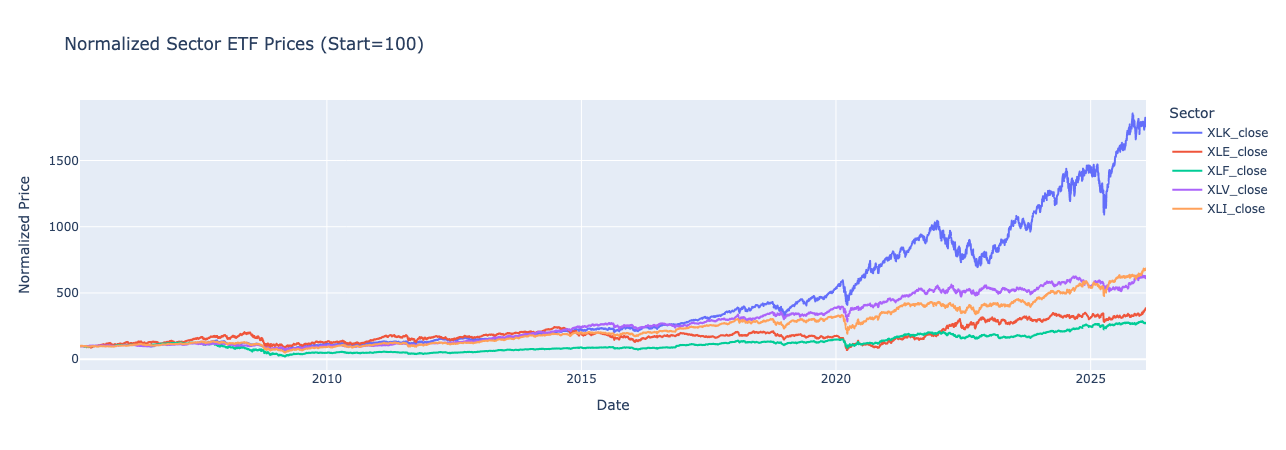
\includegraphics[width=0.95\linewidth]{normalized_sector_etf_prices.png}
    \caption{Normalized closing prices for XLK, XLE, XLF, XLV, and XLI, indexed to 100 from 2025-2026 with vertical markers for each curated macroeconomic event. Pink dashed lines denote Monetary events; yellow dashed lines denote Geopolitical events.}
    \label{fig:norm-prices}
\end{figure}

\subsubsection{30-Day Rolling Volatility.}
Figure~\ref{fig:rolling-vol} displays a plot of the rolling standard deviation of log returns for all five sectors over a rolling window of 30 days, annualized. This type of visualization highlights areas where market stress is high and allows for a comparison of the magnitude of the volatility for each sector. There are three distinct peaks in the rolling standard deviation for all five sectors: one around the financial crisis of 2008, one around the COVID-19 market shock in 2020, and one around the 2022 tightening cycle.

\begin{figure}[H]
    \centering
    \includegraphics[width=\linewidth]{30_day_annualized_rolling_volatility.png}
    \caption{30-day annualized rolling standard deviation of log returns for all five sector ETFs, 2005--2026.}
    \label{fig:rolling-vol}
\end{figure}

\subsubsection{Sector Heterogeneous Event Response.} 
Figure~\ref{fig:het-response} displays a plot of the cumulative log returns for each sector over a rolling window of 30 days (22 trading days) after each of the nine curated events. By displaying all five sectors side by side for each event, we are able to compare heterogeneous responses for each sector after the same macroeconomic event occurs, answering Research Questions 1 and 3.

\begin{figure}[H]
    \centering
    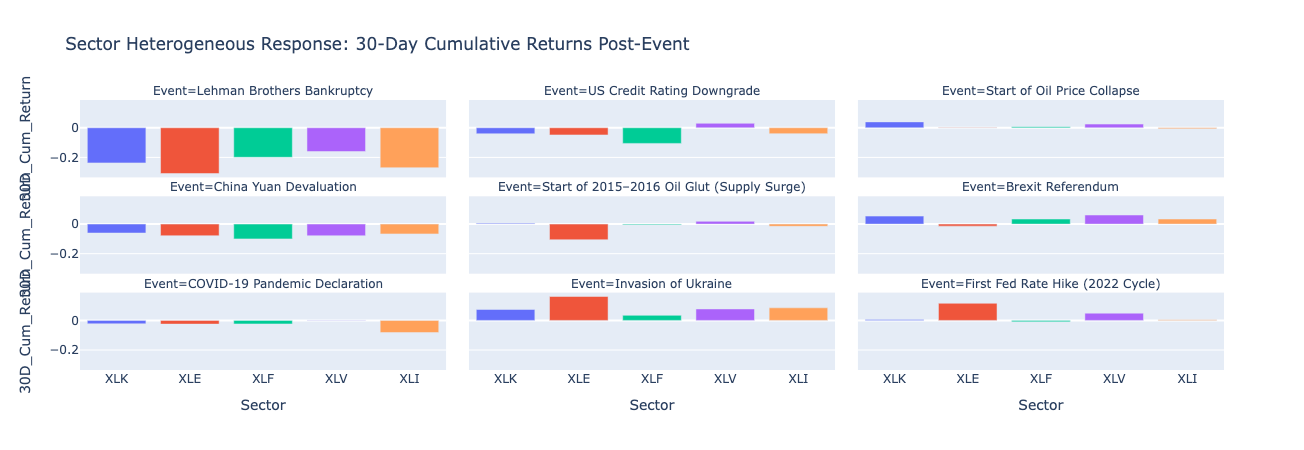
\includegraphics[width=\linewidth]{sector_heterogenous_response.png}
    \caption{30-day cumulative log returns for each sector ETF in the 22 trading days following each of the nine curated macroeconomic events.}
    \label{fig:het-response}
\end{figure}


\subsubsection{Rolling Correlation with Federal Funds Rate.}
Figure~\ref{fig:rolling-corr} presents the 6-month (126-day) rolling Pearson correlation between the log returns of each sector and FEDFUNDS. This plot directly answers Research Question 5 because we are able to visualize the evolution of sector sensitivity to monetary policy over time.

\begin{figure}[H]
    \centering
    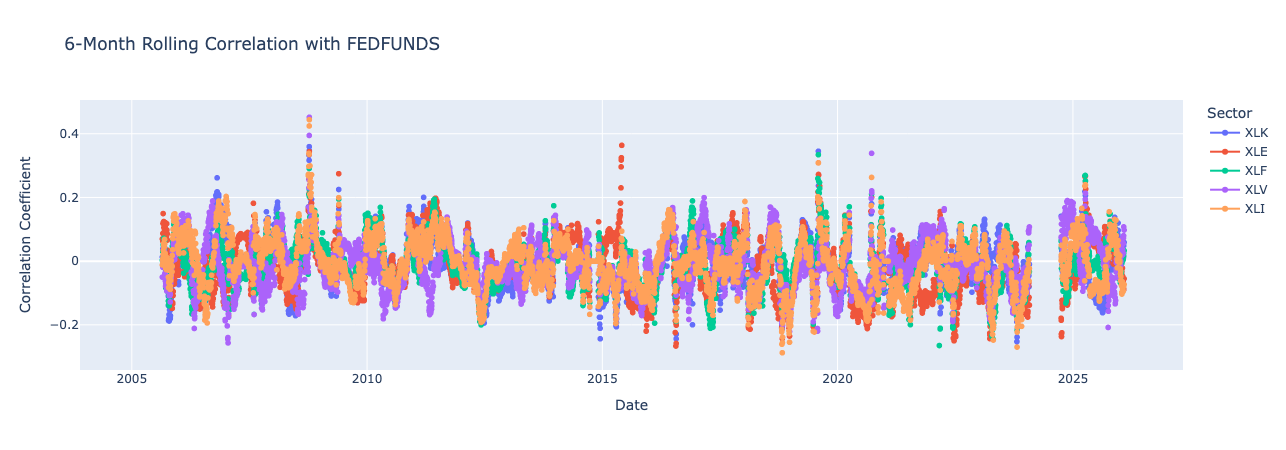
\includegraphics[width=\linewidth]{6_month_rolling_correlation_with_FEDFUNDS.png}
    \caption{6-month rolling Pearson correlation between sector log returns and the Federal Funds Effective Rate, 2005--2026.}
    \label{fig:rolling-corr}
\end{figure}

\subsubsection{Sector Correlation Heatmap.}
Figure~\ref{fig:corr-heatmap} presents the entire sample period's pairwise Pearson correlation matrix for the five sector ETFs, with an average correlation of 0.569. All sectors are positively correlated with one another. XLF and XLI have the largest correlation (0.83) as well as XLK and XLI (0.78). XLV has the lowest correlation with the other sectors (0.44) on average, as expected given its defensive nature, and XLE has the second lowest correlation (0.50) due to its commodity-driven nature. This plot, in combination with the heterogeneous event response plot, answers Research Question 6 because we can visualize the lack of diversification benefit within the sector ETFs, which diminishes even further in a systemic shock event.

\begin{figure}[H]
    \centering
    \includegraphics[width=\linewidth]{sector_correlation.png}
    \caption{Full-period pairwise Pearson correlation matrix of log returns across all five sector ETFs, 2005--2026.}
    \label{fig:corr-heatmap}
\end{figure}

\subsection{Modelling/Analytical Approach}

Three models were implemented to address our fourth Research Question and to power the dashboard's forecasting views.

% I cannot find a reference on why ARIMA 101 is the best configuration for financial time series. I'll ask chat tmw, the citations might not be correct, so we gotta double check those. 
% I feel like we can get rid of that last sentence, but I wanted to make sure. ANSWER: ARIMA is the baseline statistic in the dashboard.

\subsubsection{ARIMA(1,0,1) - Return Forecasting Baseline.}
the autoregressive integrated Moving Average (ARIMA) model of order $(p=1, d=0, q=1)$ was separately applied to each sector based on the training period's log return data using the arima class provided by statsmodels. the value of $d=0$ was chosen because of the stationary nature of log return data, which was validated during the preprocessing step. the choice of $(1,0,1)$ was based on convention for financial time series, as described in \cite{investopedia_arima}. the arima model was fitted once on the training data, and predictions were generated on the fly for the entire test period. arima was chosen as a baseline model for several reasons. it is a well-established model for financial return time series, it is computationally inexpensive, and it is easy to understand.

% do we compare garch output to the annualized volatility in the dashboard? i don't think i´ve seen that yet (? actually maybe i have) lol. answer: we did

\subsubsection{garch(1,1) --- volatility forecasting.}
A Generalized Autoregressive Conditional Heteroskedasticity (GARCH) model of order (1,1) was applied on the entire log returns series (training + test sets) for each sector, assuming a normal distribution for the error term, and the model was fitted via the \textit{arch} package. the volatility was extracted for the test set, and this was annualized by multiplying by $\sqrt{252}$. GARCH is a popular model for financial volatility, where periods of high volatility are clustered together. it is a widely used model for financial forecasting, where the price variation of an asset is predicted. GARCH is compared with the actual 30-day rolling volatility in the model performance dashboard tab.

%not too sure on what is dropout regularization. answer: we did it in the dashboard, its random disabling of data, we have it at 20%.
\subsubsection{long short-term memory (lstm) --- deep learning comparison.}
A many-to-one Long Short-Term Memory (LSTM) network was designed using the \texttt{tensorflow/keras} API for predicting the next day's log return based on a 60-day window of log returns in the past. The network consists of two LSTM layers with 50 units in each layer, followed by a dropout layer with a rate of 0.2 for overfitting prevention, and finally a dense layer with a single unit for the prediction. The model was configured to train for up to 50 epochs with early stopping (patience = 5) monitoring validation loss and restoring the best weights. In practice, training terminated well before the 50-epoch ceiling across all sectors, as the near-random-walk nature of daily log returns caused validation loss to plateau rapidly within the first several epochs. LSTM was used because of the potential for non-linear dependencies in the data, which are not addressed by the ARIMA model. The dropout layer was added after recognizing overfitting on the training set in early experiments. LSTM predictions are displayed in the model performance tab of the dashboard, given pre-computed predictions are available.

\subsubsection{evaluation metric --- rmse.}
all return-forecasting models were evaluated using root mean squared error:
\[
\text{rmse} = \sqrt{\frac{1}{n}\sum_{t=1}^{n}(\hat{r}_t - r_t)^2}
\]
where $\hat{r}_t$ is the predicted log return and $r_t$ is the actual log return. RMSE was computed separately for stable and shock days within the test set to characterize model robustness across market regimes. The shock regime is defined as days on which the sector's 30-day rolling annualized volatility exceeds the 90th percentile of the test-period volatility distribution for that sector.

\subsubsection{Interactive Dashboard Design.}
The primary deliverable is a Plotly/Dash web application comprising six interactive tabs, each addressing one or more research questions:

\begin{enumerate}
    \item \textbf{Price \& Event Overlay:} Normalized ETF prices with selectable sectors and filterable event category markers (Monetary / Geopolitical / All).
    \item\textbf{30-Day Rolling Volatility:} 30-day annualized rolling standard deviation of log returns for all five sectors, with selectable sectors and filterable event category markers (Monetary / Geopolitical / All).
    \item \textbf{Event Drill-Down:} Cumulative 22-trading-day log returns and normalized price trajectories following a user-selected event.
    \item \textbf{Model Performance:} Backtested ARIMA and LSTM return predictions versus actuals, with GARCH conditional volatility versus actual rolling volatility, and red shading for shock regime periods.
    \item \textbf{Rolling Correlation with FEDFUNDS:} Rolling Pearson correlation between each sector's log returns and FEDFUNDS, with user-selectable windows of 3, 6, or 12 months.
    \item \textbf{Sector Relationships:} Pairwise Pearson correlation heatmap across the five sectors, computed over a user-defined date range (year and month selectors) with a market regime filter (All / Stable / Shock). 
    \item \textbf{Future Outlook:} Forward price projection using ARIMA for the mean trajectory and GARCH-based cumulative variance for 95\% confidence intervals, over a user-selected horizon of 20--126 trading days.
\end{enumerate}

% ═══════════════════════════════════════════════════════════════════════════════
\section{Results}

% RQ1
\subsection{30-Day Cumulative Returns Following Macro Events}

Figure~\ref{fig:het-response} displays the 30-day cumulative log return for each of the five sectors in the 22 trading days immediately following each of the nine selected events. The magnitudes and signs of cumulative returns differ across sectors for the same event. The Lehman Brothers Bankruptcy produces the largest uniform drop, with all five sectors recording cumulative returns between $-0.20$ and $-0.25$. Following the Invasion of Ukraine (February 24, 2022), XLE records a strongly positive cumulative return while the remaining four sectors record negative values. Following the First Fed Rate Hike of the 2022 cycle, XLK records the most negative value, while XLF remains close to zero. Across nearly all nine events, XLV records among the smallest absolute cumulative returns.

% RQ2
\subsection{30-Day Rolling Volatility}

Figure~\ref{fig:rolling-vol} shows three prominent annualized volatility spikes across all sectors: the 2008--2009 financial crisis, the March 2020 COVID-19 shock, and the 2022 tightening cycle. XLE consistently exhibits the highest peak volatility of any sector during commodity-driven episodes, including the 2014--2016 oil price collapse and the 2022 period, where its annualized rolling volatility substantially exceeds that of the other four sectors. XLV records the lowest and most stable rolling volatility throughout the full period, rarely exceeding levels reached by the other sectors outside of systemic shock windows. Geopolitical events tend to produce sharper, shorter-lived volatility spikes, while the 2022 monetary tightening cycle produced a more prolonged elevation across all sectors.

% RQ3
\subsection{Asymmetric Sector Recovery}

The 22-day pre- and post-event price chart in the Event Drill-Down tab reveals asymmetric recovery patterns across sectors. Following the Lehman Brothers Bankruptcy, all sectors declined sharply in the days following the event but show divergent trajectories over the subsequent 22 days, with XLV stabilizing faster than XLE and XLF. Following the Ukraine Invasion, XLE recovers and appreciates immediately while other sectors remain below their pre-event levels, illustrating a case where a geopolitical shock produced asymmetric cross-sectional outcomes rather than a uniform decrease and recovery. Supply-side energy shocks (Oil Glut, 2015--2016) show XLE continuing to decline over the post-event window while all other sectors stabilize, indicating that sector-specific shocks produce more persistent one-directional moves than systemic ones.

% RQ4
\subsection{Forecasting Performance}

Table~\ref{tab:regime_rmse} reports the RMSE for ARIMA(1,0,1) and LSTM models evaluated on the 2024--2026 test set (546 trading-day observations per sector), stratified by stable and shock regimes.

\begin{table}[H]
\centering
\caption{Regime-based RMSE for ARIMA(1,0,1) and LSTM on the 2024--2026 test set (546 observations per sector). Shock regime is defined as days exceeding the 90th percentile of test-period rolling 30-day annualized volatility.}
\label{tab:regime_rmse}
\begin{tabular}{lcccc}
\toprule
\textbf{Sector} & \textbf{ARIMA (Stable)} & \textbf{ARIMA (Shock)} & \textbf{LSTM (Stable)} & \textbf{LSTM (Shock)} \\
\midrule
XLK & 0.01303 & 0.02860 & 0.01346 & 0.02927 \\
XLE & 0.01125 & 0.02599 & 0.01543 & 0.02877 \\
XLF & 0.00857 & 0.02038 & 0.00882 & 0.02073 \\
XLV & 0.00778 & 0.01594 & 0.00789 & 0.01610 \\
XLI & 0.00836 & 0.02007 & 0.00844 & 0.02025 \\
\bottomrule
\end{tabular}
\end{table}

\noindent Across all five sectors and both market regimes, the ARIMA(1,0,1) model records a lower RMSE than the LSTM. The largest absolute difference occurs in the XLE stable regime, where the LSTM RMSE (0.01543) is approximately 37\% higher than ARIMA (0.01125). XLV records the lowest RMSE of any sector in both regimes and for both models. Shock-regime RMSE is persistently larger than stable-regime RMSE across every sector-model combination; the shock-to-stable ratio for ARIMA ranges from 2.05 (XLV) to 2.31 (XLF), which indicates that prediction errors approximately double during high-volatility periods.

% RQ5
\subsection{Rolling Correlation with the Federal Funds Rate}

Figure~\ref{fig:rolling-corr} displays the 6-month rolling Pearson correlation between each sector's log returns and the FEDFUNDS series over the full 2005--2026 window. For most of the 2010--2019 period, all five sectors maintained rolling correlations close to zero, reflecting the low and stable rate environment. During the 2022--2023 tightening cycle, XLK and XLF shift toward more negative correlations, consistent with increasing interest rate sensitivity, while XLE went in the opposite direction, recording positive correlations as energy prices and rates moved together during that period.

% RQ6
\subsection{Sector Relationships}

Figure~\ref{fig:corr-heatmap} shows that all pairwise Pearson correlations among the five sectors are positive over the full period, with an average of 0.569. XLF--XLI (0.83) and XLK--XLI (0.78) exhibit the strongest co-movement. XLV records the lowest sector average correlation (0.44) and XLE the second lowest (0.50), reflecting their respective defensive and commodity-driven characteristics. The regime filter in the dashboard reveals that correlations rise substantially during shock periods, with the average correlation approaching one during significant events such as the 2008 crisis.

% RQ7
\subsection{Forecast Uncertainty}

The Future Outlook tab generates forward price projections combining ARIMA mean forecasts with GARCH-based 95\% confidence intervals over user-selectable horizons of 20--126 trading days. The width of the uncertainty cone varies materially across sectors. XLE and XLK produce the widest confidence intervals, consistent with their higher historical return volatility. XLV produces the narrowest cone, consistent with its lower rolling volatility and RMSE across the test period. For all sectors, the confidence interval widens substantially with horizon length due to the accumulation of GARCH-modeled variance, confirming that medium-term sector price paths carry significant uncertainty even under the best-performing model.

% ═══════════════════════════════════════════════════════════════════════════════
\section{Discussion}
%RQ1
\subsection{Sector-Specific Event Responses}

As seen from the 30-day cumulative return patterns following macroeconomic events (Figure~\ref{fig:het-response}), the response of different sectors to the same macro event is heterogeneous in both sign and magnitude. The large and widespread drawdown after the Lehman Brothers Bankruptcy highlights the nature of that event as a systemic financial crisis. The positive response of XLE to the Ukraine Invasion highlights that geopolitical shocks affecting commodities can generate sector-level winners and losers rather than uniform market declines. These cross-sectional differences are consistent with previous evidence that macroeconomic shocks transmit unevenly across industries \cite{ewing2003, ewing2002} and supports the use of sector-level analysis rather than aggregate market indices when assessing the impact of macro events.

%RQ2 chat hallucinated a quote here
\subsection{Volatility Dynamics Across Sectors and Shock Types}

The rolling annualized volatility patterns (Figure~\ref{fig:rolling-vol}) show that sector volatility is both time-varying and depends on the type of shock experienced in the market. For example, financial crises and global health events (2008--2009, COVID-19) generate volatility spikes across all sectors, whereas commodity-specific shocks (e.g., the 2014--2016 oil collapse, the 2022 energy shock) are felt mostly in XLE. XLV’s persistently lower and more stable volatility is consistent with its characterization as a defensive sector in the literature, which typically shows that healthcare and consumer staples are less affected by the business cycle \cite{sprague2024healthcare}. The contrast between shorter-lived volatility spikes around geopolitical events and the more prolonged elevation during the 2022 tightening cycle suggests that monetary regimes can alter the baseline risk environment for long periods, as highlighted in literature on the impact of monetary policy on equity markets \cite{ewing2003}.

%RQ3
\subsection{Asymmetric Recovery Patterns}

The event-level drill-downs show that drawdowns and recoveries are not symmetric over time and across sectors. The faster stabilization of XLV following the Lehman Brothers Bankruptcy and the prolonged decline of XLE following the Oil Glut episode suggest that sector-specific mechanisms, such as regulated demand in healthcare versus commodity price exposure in energy—related sectors, affect recovery patterns. The immediate appreciation of XLE following the Ukrainian Invasion, alongside the persistent underperformance of other sectors, illustrates that certain shocks can trigger positive re-pricing in affected industries while leaving the broader market unaffected. These findings reflect prior evidence that sector adjustments to macroeconomic shocks exhibit heterogeneity not only in impact magnitude but also in recovery speed \cite{ewing2003}, with implications for timing strategies around event windows.

%RQ4
\subsection{Predictive Performance Across Regimes}

The regime-stratified RMSE results (Table~\ref{tab:regime_rmse}) reinforce two key points. First, a relatively simple linear benchmark (ARIMA(1,0,1)) outperforms the more complex LSTM across all sectors and regimes in this implementation. Given that the LSTM's early stopping (patience = 5) triggered within the first several epochs despite a 50-epoch ceiling, this gap is plausibly attributable to undertraining rather than an inherent inferiority of neural networks. This aligns with a broad literature showing that complex models require careful adjustments and sufficient data to surpass well-specified statistical baselines in financial forecasting.
\vspace{0.5cm}
Second, the systematic increase in RMSE during high-volatility “shock” regimes (roughly doubling relative to stable periods across all sector and model combinations) confirms that forecast precision deteriorates when macro uncertainty is elevated. This pattern is consistent with Ewing et al.\ \cite{ewing2003}, who document heterogeneous and pronounced sector responses to macroeconomic disturbances. Our results extend that insight to a forecasting context: model error is regime-dependent, with periods of greatest market stress coinciding with the greatest predictive uncertainty.

%RQ5
\subsection{Monetary Policy Sensitivity}

The evolution of rolling correlations between sector returns and the Federal Funds Rate (Figure~\ref{fig:rolling-corr}) suggests that interest-rate sensitivity is both time-varying and regime-specific. Near-zero correlations during the 2010--2019 low-rate environment indicate limited information content of policy changes for sector returns in that regime. By contrast, the 2022--2023 tightening cycle coincides with more negative correlations for technology (XLK) and financials (XLF), and a positive shift for energy (XLE), consistent with concurrent increases in both rates and commodity prices. These patterns are in line with prior evidence that monetary policy shocks exert their strongest influence on financially levered and capital-intensive sectors \cite{ewing2003}, while also highlighting an evolving interest-rate sensitivity for growth-oriented technology stocks in the post-pandemic period. A formal structural-break analysis would be ideal to confirm whether this reflects a persistent regime shift.

%RQ6
\subsection{Cross-Sector Correlations and Diversification}

The cross-sector correlation structure (Figure~\ref{fig:corr-heatmap}) shows that, on average, all pairwise correlations are positive, with especially strong co-movement among cyclical sectors such as Financials and Industrials. XLV and XLE exhibit relatively lower average correlations, consistent with the notion that defensive and commodity-driven sectors occupy less impacted positions during market shocks \cite{ewing2002}. The marked rise in correlations during systemic shock periods, with average values approaching one, implies that diversification benefits within the observed sectors diminish precisely when investors most rely on them. From a portfolio-construction perspective, these results caution against overrelying on static sector diversification and highlight the need for regime-aware risk management.

%RQ7
\subsection{Forecast Uncertainty and Sector Risk Profiles}

The forecasting model-based uncertainty cones derived from ARIMA–GARCH forecasts reveal that forecast dispersion differs systematically across sectors and horizons. Wider cones for XLE and XLK reflect their higher realized volatility and larger forecast errors, while the narrower one developed for XLV is consistent with its more stable return profile and lower RMSE. The rapid widening of confidence intervals over longer horizons illustrates the compounding effect of volatility on forecast uncertainty, reflecting the fact that return predictability falls the more we observe in the future in equity markets. These results emphasize that forward-looking sector risk is not uniform and that even under the best-performing model, medium-term price paths remain highly uncertain, particularly for commodity-exposed sectors.

\subsection{Limitations}
%This section is very good
\begin{itemize}
    \item \textbf{LSTM Convergence:} Although the LSTM was configured for up to 50 epochs, early stopping (patience = 5) caused training to terminate within the first several epochs across all sectors, as validation loss plateaued rapidly on near-random-walk return data. The reported LSTM RMSEs therefore do not reflect the model's potential capability under more expressive input features or a richer training configuration.

    \item \textbf{Static Event List:} The nine curated events represent a manually selected and fixed set of shocks. This introduces selection bias and does not capture the full universe of market-moving news. A dynamic, automated event sourcing approach (e.g., a fully curated Wikidata pipeline or NLP-based news feed) would improve generalizability.

    \item \textbf{ARIMA Linearity Assumption:} ARIMA assumes linear dependencies in the return series. Financial returns exhibit well-documented nonlinearities (e.g., leverage effects, tail dependence) that ARIMA cannot capture, which may partially explain the elevated RMSE during shock regimes.

    \item \textbf{GARCH Evaluation:} GARCH volatility forecasts were evaluated visually against rolling realized volatility but were not subjected to formal hypothesis tests (e.g., Diebold--Mariano) due to scope constraints. Formal statistical comparison of volatility models remains a direction for future work.

    \item \textbf{Sector Coverage:} The five ETFs analyzed (XLK, XLE, XLF, XLV, XLI) represent a subset of the eleven GICS sectors. Sectors such as Real Estate (XLRE), Consumer Discretionary (XLY), and Materials (XLB) were excluded, limiting the transferability of cross-sector findings.
\end{itemize}

\subsection{Future Directions}

\begin{itemize} %These are hypothetical RIGHT? ANSWER: Yes, I believe it is hypothetical
    \item \textbf{Full LSTM Training:} Retraining the LSTM for 50--100 epochs with validation-based early stopping and hyperparameter tuning (learning rate, batch size, sequence length) is the most immediate improvement available and could substantially close the performance gap with ARIMA.

    \item \textbf{Multivariate Models:} The strong cross-sector correlations observed in the heatmap motivate extending the forecasting framework to multivariate models such as VAR-GARCH or multivariate LSTM, which could exploit inter-sector dependencies as predictive features.

    \item \textbf{Formal Statistical Testing:} Applying Diebold--Mariano tests for return forecasts and Kupiec or Christoffersen tests for volatility interval forecasts would position our model comparison in a statistically defensible place.
    
    \item \textbf{Real-Time Data Integration:} The dashboard's architecture is compatible with live data feeds via the Alpha Vantage API, which would enable near-real-time monitoring of sector dynamics without retraining.

    \item \textbf{Expanded Sector Coverage:} Adding all eleven GICS sector ETFs and conducting sector-rotation analysis across monetary policy cycles would extend the practical relevance of the platform for portfolio construction.
\end{itemize}

% ═══════════════════════════════════════════════════════════════════════════════
\section{Conclusion}

\noindent This project delivered an end-to-end forecasting and market analysis platform for five U.S.\ equity sector ETFs spanning 21 years (2005--2026), structured around seven research questions and operationalized through a seven-tab interactive Plotly/Dash dashboard. By combining ARIMA(1,0,1), GARCH(1,1), and LSTM forecasting with regime-stratified evaluation, rolling correlation analysis, cross-sector relationship mapping, and asymmetric event recovery visualization, the project produced a comprehensive analytical framework for understanding how sector ETFs behave across different macroeconomic regimes.

\hfill

\noindent The key empirical findings are as follows. First, sector returns respond heterogeneously to macroeconomic shocks (RQ1), with the pre/post event symmetric window revealing that recovery trajectories diverge substantially across sectors and are not symmetric around the shock date (RQ3). Second, XLE's 30-day rolling volatility exhibits pronounced spikes during supply shocks that are absent in other sectors, while XLV's volatility remains consistently suppressed (RQ2). Third, ARIMA outperforms LSTM across all five sectors, with shock-regime RMSE consistently two to three times larger than stable-regime RMSE; LSTM performance is limited by early stopping, which triggered within approximately five epochs due to near-random-walk log return dynamics (RQ4). Fourth, XLE's rolling correlation with the Federal Funds Rate splits sharply during 2022--2023, while XLF and XLK show the strongest positive co-movement with rate changes (RQ5). Fifth, the sector correlation heatmap reveals a diversification illusion: the average pairwise Pearson correlation across sectors is 0.569, with XLF--XLI reaching 0.83 and XLV maintaining the lowest average at 0.44 --- indicating meaningful but limited diversification benefit (RQ6). Finally, GARCH-modeled conditional volatility in the Future Outlook tab confirms that forecast uncertainty is regime-dependent and highest during identified shock windows (RQ7), consistent with \cite{ewing2003} and \cite{ewing2002}.

\hfill

\noindent The resulting dashboard makes these findings accessible without requiring specialist quantitative finance knowledge, supporting both exploration and structured research inquiry. Future extensions include full LSTM training with multivariate inputs, expanded sector coverage, real-time data integration, and sentiment-augmented forecasting.

\hfill
\pagebreak

% ═══════════════════════════════════════════════════════════════════════════════
\begin{thebibliography}{}

\bibitem{cfadata2024}
CFA Institute. (2024, March 22). \textit{Why data science is a key skill for investment professionals}. https://www.cfainstitute.org/

\bibitem{alomari2024}
Alomari, M., Selmi, R., Mensi, W., Ko, H., \& Kang, S. H. (2024). Dynamic spillovers in higher moments and jumps across ETFs and economic and financial uncertainty factors in the context of successive shocks. \textit{The Quarterly Review of Economics and Finance, 93}, 210--228. https://doi.org/10.1016/j.qref.2023.12.009

\bibitem{stooq}
Stooq. (n.d.). \textit{Stooq historical market data}. https://stooq.com/db/h/

\bibitem{fred}
Federal Reserve Bank of St.\ Louis. (n.d.). \textit{Federal funds effective rate} [FEDFUNDS]. FRED. https://fred.stlouisfed.org/series/FEDFUNDS

\bibitem{syllabus}
DATA 501. (2026). \textit{CAT-2.1: Stock market trend forecasting dashboard}. Course syllabus and project description, Winter 2026.

\bibitem{investopedia_arima}
Investopedia. (2025, August 7). \textit{Autoregressive integrated moving average (ARIMA)}. https://www.investopedia.com/terms/a/autoregressive-integrated-moving-average-arima.asp

\bibitem{quantstart_garch}
Investopedia. (2024, July 15). \textit{Generalized autoregressive conditional heteroskedasticity (GARCH)}. https://www.investopedia.com/terms/g/garch.asp


\bibitem{sahaf2017}
Sahaf, Z., Marbouti, M., Mota, R. C., Alemasoom, H., Maurer, F., \& Sousa, M. C. (2017). PipeVis: Interactive visual exploration of pipeline incident data. In \textit{EuroVis Workshop on Visual Analytics (EuroVA)} (pp. 31--35).

\bibitem{ewing2003}
Ewing, B. T., Forbes, S. M., \& Payne, J. E. (2003). The effects of macroeconomic shocks on sector-specific returns. \textit{Applied Economics, 35}(2), 201--207.

\bibitem{ewing2002}
Ewing, B. T. (2002). The transmission of shocks among S\&P indexes. \textit{Applied Financial Economics, 12}(4), 285--290.

\bibitem{progress}
Frese, A., Reyes González, K., \& Elbouni, W. (2026). \textit{Progress report: Interactive dashboard for analysis and forecasting of sector performance}. DATA 501 Capstone, Winter 2026.

\bibitem{sprague2024healthcare}
Sprague, A. (2024).
Health care sector report.\textit{Investment Management Program, John L. Grove College of Business, Shippensburg University}.


\end{thebibliography}

\newpage

% ═══════════════════════════════════════════════════════════════════════════════
\appendix
\section{Data Pipeline Overview}

The full data pipeline is implemented in Python and organized as a modular script (\texttt{app.py}) at the repository root. The pipeline proceeds in the following order:

\begin{enumerate}
    \item \textbf{Data Loading:} The master sector dataset (\texttt{data/processed/master\_sector\_data.csv}) is loaded with a DatetimeIndex and aligned to business-day frequency with forward-fill.
    \item \textbf{Prediction Loading or Generation:} Pre-computed model predictions are loaded from \texttt{data/processed/model\_predictions.csv} if available. If the file is absent or missing the \texttt{garch\_vol} column, ARIMA(1,0,1) and GARCH(1,1) predictions are generated on-the-fly for each sector and saved.
    \item \textbf{Event Definition:} The nine curated events are defined as a Python list of dictionaries and converted to a Pandas DataFrame with parsed dates.
    \item \textbf{Dashboard Construction:} The Dash application layout is built using Dash Mantine Components with seven interactive tab panels. Each tab is connected to one or more callbacks that reactively update figures based on user selections.
\end{enumerate}

\noindent Key code excerpt for ARIMA and GARCH fitting (pseudocode):
\begin{verbatim}
for sector in ["XLK", "XLE", "XLF", "XLV", "XLI"]:
    arima = ARIMA(train_log_ret[sector], order=(1,0,1)).fit()
    arima_preds = arima.predict(start=test_start, end=test_end)

    garch = arch_model(full_log_ret[sector], vol="Garch",
                       p=1, q=1).fit(disp="off")
    garch_vol = garch.conditional_volatility * sqrt(252)
\end{verbatim}

\section{Dashboard Tab Reference}

\begin{table}[H]
\centering
\caption{Summary of the seven interactive dashboard tabs, their Dash callback IDs, and the research questions they address.}
\begin{tabular}{llp{4.5cm}c}
\toprule
\textbf{Tab} & \textbf{ID} & \textbf{Description} & \textbf{RQ(s)} \\
\midrule
Price \& Event Overlay   & \texttt{overlay}      & Normalized prices with filterable event markers       & 1, 2 \\
30-Day Rolling Volatility& \texttt{volatility}   & Annualized rolling vol with event overlays            & 2    \\
Event Drill-Down         & \texttt{events}       & Cum.\ returns and pre/post price paths around events  & 1, 3 \\
Model Performance        & \texttt{performance}  & ARIMA/LSTM returns; GARCH vs.\ realized vol           & 4    \\
Rolling Correlation      & \texttt{corr}         & Sector--FEDFUNDS rolling Pearson correlation          & 5    \\
Sector Relationships     & \texttt{relationships}& Pairwise sector correlation heatmap with regime filter& 6    \\
Future Outlook           & \texttt{future}       & ARIMA forecast + GARCH 95\% CI forward projection     & 7    \\
\bottomrule
\end{tabular}
\end{table}

\section{All Computations/Code}

\subsection{Data Preprocessing (\texttt{src/preprocessing.py})}       

\lstinputlisting[language=Python]{preprocessing_listing.py}            

\subsection{Dashboard Application (\texttt{app.py})}

\lstinputlisting[language=Python]{app_listing.py}

\subsection{Data Acquisition and Preprocessing (\texttt{notebooks/1\_data\_acquisition.ipynb})}

\lstinputlisting[language=Python]{1_data_acquisition_listing.py}

\subsection{Exploratory Data Analysis (\texttt{notebooks/2\_exploratory\_analysis.ipynb})}

\lstinputlisting[language=Python]{2_exploratory_analysis_listing.py}

\subsection{Modelling and Forecasting (\texttt{notebooks/3\_modeling\_forecasting.ipynb})}

\lstinputlisting[language=Python]{3_modeling_forecasting_listing.py}

\end{document}
